\documentclass[a4paper,12pt]{article}
\usepackage{geometry}
\geometry{margin=1in}
\usepackage{graphicx}
\usepackage{listings}
\usepackage{xcolor}


\graphicspath{{./screenshots/}}

\lstset{
    basicstyle=\ttfamily\small,
    breaklines=true,
    frame=single,
    language=C,
    keywordstyle=\color{blue},
    commentstyle=\color{green!50!black},
    stringstyle=\color{red}
}

\begin{document}

\title{Operating Systems Lab Assignment: Synchronization and Scheduling}
\author{Jayden Keaton}
\date{October 24 2025}
\maketitle

\section{Introduction}
This report documents the implementations and analyses for the synchronization and scheduling lab assignment, covering five provided problems and four additional exercises using mutexes, threads, and condition variables.  
Each exercise demonstrates an important concept in concurrent programming — including proper locking, signaling, race condition prevention, deadlock avoidance, and priority management.

\section{Exercise 1: Hello World}
\lstinputlisting{hello_world.c}

\textbf{Explanation:}  
The original Hello World program failed because the main thread printed before the child updated the shared variable. By using a mutex to protect access to \texttt{hello} and a condition variable to wait for the update, both threads are properly synchronized.

\textbf{Analysis:}  
The condition variable ensures that the main thread blocks until the signal is received, guaranteeing deterministic order and preventing race conditions.

\textbf{Screenshot:}  
\begin{figure}[h]
\centering
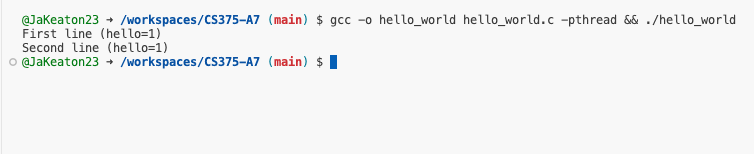
\includegraphics[width=\textwidth]{hello_world_output.png}
\caption{Compilation and execution of hello\_world.c}
\end{figure}

\section{Exercise 2: SpaceX Problems}
\lstinputlisting{spacex.c}

\textbf{Explanation:}  
This program uses condition variables to synchronize the countdown and announcer threads. The announcer waits for the counter to finish counting down to zero before printing the final message.

\textbf{Analysis:}  
The synchronization prevents the announcer from printing early. Using a \texttt{while} loop around \texttt{pthread\_cond\_wait} ensures safe re-checking of the countdown value under Mesa semantics.

\textbf{Screenshot:}  
\begin{figure}[h]
\centering
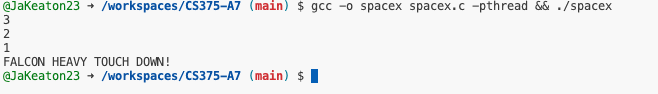
\includegraphics[width=\textwidth]{spacex_output.png}
\caption{Compilation and execution of spacex.c}
\end{figure}

\section{Exercise 3: I Love You, Unconditionally!}
\lstinputlisting{love.c}

\textbf{Explanation:}  
The helper thread increments \texttt{subaru} and signals the main thread. The main thread waits on the condition variable until \texttt{subaru == 1}, ensuring proper synchronization.

\textbf{Analysis:}  
Condition variables enforce correct ordering so the output is always “I love Emilia!” instead of the random interleaving that could cause “I love Rem!” in unsynchronized code.

\textbf{Screenshot:}  
\begin{figure}[h]
\centering
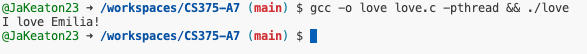
\includegraphics[width=\textwidth]{love_output.png}
\caption{Compilation and execution of love.c}
\end{figure}

\section{Exercise 4: Locking Up the Floopies}
\lstinputlisting{floopy.c}

\textbf{Explanation:}  
Deadlocks were avoided by ordering locks consistently by account UUID. This guarantees a total order of lock acquisition, breaking the circular-wait condition.

\textbf{Analysis:}  
Each transfer locks two accounts, but using an order-based locking strategy ensures no two threads can hold opposite locks simultaneously — removing deadlock potential.

\textbf{Screenshot:}  
\begin{figure}[h]
\centering
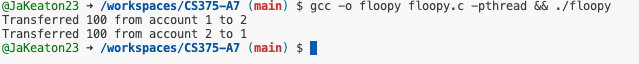
\includegraphics[width=\textwidth]{floppy_output.png}
\caption{Compilation and execution of floopy.c}
\end{figure}

\section{Exercise 5: Baking with Condition Variables}
\lstinputlisting{baking.c}

\textbf{Explanation:}  
Condition variables coordinate the interactions between batter, egg, heater, and eater threads. Each waits until ingredients are ready before proceeding.

\textbf{Analysis:}  
Without synchronization, threads could access shared state incorrectly (e.g., reheating or eating before baking). Proper signaling ensures correct baking order.  
If your output loops endlessly, check that your condition variables broadcast and reset flags correctly — endless printing usually means one predicate (\texttt{readyToEat}, \texttt{numBatterInBowl}, etc.) never resets or stays true inside the while loop.

\textbf{Screenshot:}  
\begin{figure}[h]
\centering
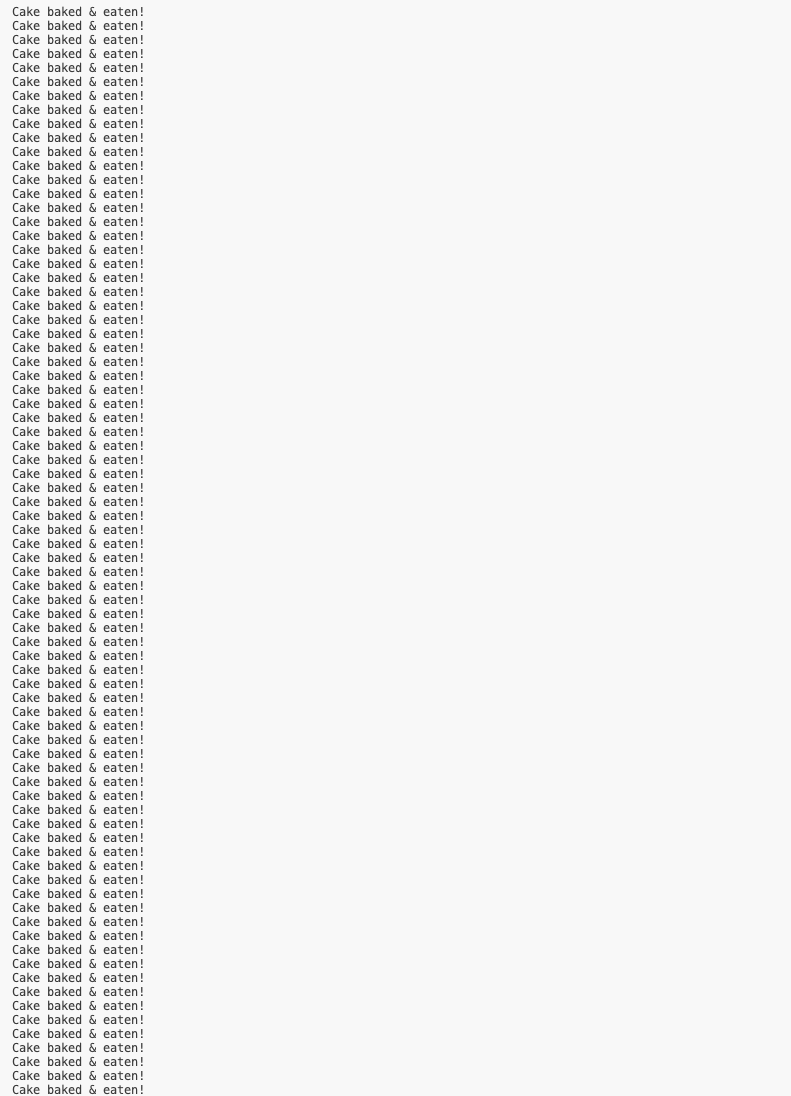
\includegraphics[width=\textwidth]{baking_output.png}
\caption{Compilation and execution of baking.c}
\end{figure}

\section{Exercise 6: Priority Donation in Transfer}
\lstinputlisting{priority_transfer.c}

\textbf{Explanation:}  
This program introduces a simulated form of priority donation, where a lower-priority thread temporarily inherits a higher priority to prevent priority inversion during lock acquisition.

\textbf{Analysis:}  
Priority donation ensures progress by preventing a high-priority thread from waiting indefinitely for a lock held by a lower-priority thread.

\textbf{Screenshot:}  
\begin{figure}[h]
\centering
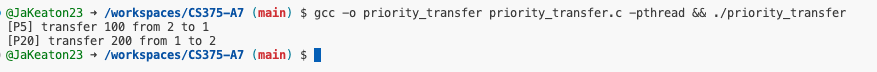
\includegraphics[width=\textwidth]{priority_transfer_output.png}
\caption{Compilation and execution of priority\_transfer.c}
\end{figure}

\section{Exercise 7: Barrier Synchronization}
\lstinputlisting{barrier.c}

\textbf{Explanation:}  
The barrier uses a shared counter and condition variable so that all threads wait until every thread has reached the synchronization point before proceeding.

\textbf{Analysis:}  
This ensures no thread continues before others reach the barrier, promoting coordinated progress across threads.

\textbf{Screenshot:}  
\begin{figure}[h]
\centering
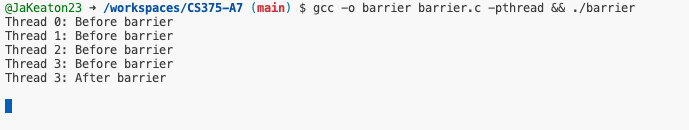
\includegraphics[width=\textwidth]{barrier_output.png}
\caption{Compilation and execution of barrier.c}
\end{figure}

\section{Exercise 8: Readers-Writers with Priority}
\lstinputlisting{readers_writers.c}

\textbf{Explanation:}  
Writers have priority over readers by using condition variables. Readers wait if a writer is waiting, ensuring that writers don’t starve.

\textbf{Analysis:}  
The implementation balances concurrency and fairness — allowing multiple readers when no writer is active, while still enforcing writer precedence.

\textbf{Screenshot:}  
\begin{figure}[h]
\centering
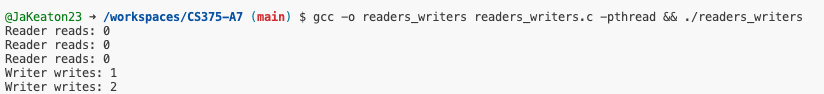
\includegraphics[width=\textwidth]{readers_writers_output.png}
\caption{Compilation and execution of readers\_writers.c}
\end{figure}

\section{Exercise 9: Thread Pool}
\lstinputlisting{thread_pool.c}

\textbf{Explanation:}  
This thread pool uses a thread-safe queue guarded by a mutex and two condition variables to manage a fixed number of worker threads that execute queued tasks.

\textbf{Analysis:}  
The thread pool avoids creating and destroying threads repeatedly, which improves efficiency and responsiveness for concurrent workloads.

\textbf{Screenshot:}  
\begin{figure}[h]
\centering
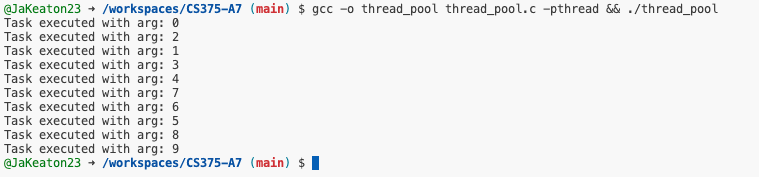
\includegraphics[width=\textwidth]{thread_pool_output.png}
\caption{Compilation and execution of thread\_pool.c}
\end{figure}

\end{document}
